\texttt{Consegna:}
\begin{enumerate}
    \item Caricamento e visualizzazione modelli mesh poligonali
    \begin{enumerate}
        \item Caricamento e visualizzazione di più di un oggetto mesh con la possibilità di passare la selezione dall'uno all'altro tramite special key
        \item Verifica della gestione della visualizzazione dei modelli poligonali tramite VAO/VBO
        \item Calcolo e memorizzazione delle normali ai vertici per i modelli mesh poligonali. Visualizzazione con normali ai vertici in modalità smooth
        \item Permettere il cambio di materiale dell'oggetto da pop-up menù
    \end{enumerate}
    \item Navigazione interattiva in scena
    \begin{enumerate}
        
        \item Pan orizzontale camera
        \item Pan verticale camera
        \item Zoom camera
        \item Culling
        \item Smooth/Flat shading
        \item Materials
        \item Camera Motion
    \end{enumerate}
    \item Trasformazione degli oggetti in scena
    \begin{enumerate}
        \item Traslazione, Rotazione, Scalatura WCS/OCS
    \end{enumerate}
    
\end{enumerate}
\texttt{Svolgimento:}\\
Parto dal presupposto che ho dovuto commentare la generazione della sfera(luce) dal codice, perchè per una qualche ragione non ancora ben identificata, con quella matrice sul mio computer con OS Arch non visualizzo più nessun oggetto. 
Su Ubuntu invece, mi funzionava anche con quella riga di codice, sinceramente non ho capito la motivazione.\\ Inoltre, per poter testare, è necessario cambiare
il path di \textbf{MeshDir}, in quanto la mia architettura richiedeva un path assoluto e non relativo.
\begin{enumerate}
    \item Caricamento e visualizzazione modelli mesh poligonali
    \begin{enumerate}
        \item Ogni oggetto è, al momento della inizializzazione, caricato utilizzando la funzione \textit{createMesh}, che inserisce l'oggetto all'interno di un array. Il controllo di quale elemento mostrare in ogni momento, è gestito grazie alla variabile \textbf{selectedObject} e dalla funzione \textit{drawOne}
        \item Nulla da dover descrivere
        \item  La richiesta è stata implementata aumentando le funzioni \textit{generate\_and\_load\_buffers} e \textit{loadObjFile}
        \item E' stata implementata la funzione \textit{material\_menu\_function} che, dato il valore dell'opzione cliccato,
        modifica il tipo di materiale dell'oggetto in questo momento selezionato
    \end{enumerate}
    \item Navigazione interattiva in scena
    \begin{enumerate}
    
        \item Le funzioni che si occupano dello spostamento a destra e sinistra sono rispettivamente \textit{moveCameraRight} e \textit{moveCameraLeft}.
        Per risolvere la richiesta, è necessario modificare la posizione della camera e del target, di uno stesso valore. In particolare, il vettore che si occupa di quantificare lo spostamento è un vettore a 4 dimensioni con valori 1,0,-1,0. Per spostarsi a sinistra il vettore è stato sommato a quello che identifica la posizione del target e della camera, per lo spostamento a destra sono stati sottratti.
        \item Le funzioni che si occupano dello spostamento in alto e in baso sono rispettivamente \textit{moveCameraUp} e \textit{moveCameraDown}. Per risolvere la richiesta, è necessario modificare la posizione della camera e del target, di uno stesso valore. In particolare, il vettore che si occupa di quantificare lo spostamento è un vettore a 4 dimensioni con valori 1,0,-1,0. Per spostarsi in alto il vettore è stato sommato a quello che identifica la posizione del target e della camera, per lo spostamento in basso sono stati sottratti.
        \item Le funzioni che si occupano dello zoom in avanti e indietro sono rispettivamente \textit{moveCameraForward} e \textit{moveCameraBack}. L'idea delle due funzioni è la stessa, cambia solo la costante che indica il movimento, da 1 a -1. L'implementazione segue la regola della retta parametrica passante per un punto. Si prende il vettore che va dal punto target alla posizione attuale. Il valore delle componenti sarà positivo se ci si vuole avvicinare al target, negativo altrimenti. A questo punto si aggiorna la posizione sommando quella attuale con il vettore, moltiplicato per una costante che ne indica la quantità di spostamento. 
        \item E' sufficiente invocare rispettivamente \textit{glEnable} e \textit{glDisable} del valore \textbf{GL\_CULL\_FACE} per abilitare o disabilitare il culling
        \item E' sufficiente invocare \textit{gkShadeModel} con il valore \textbf{GL\_FLAT} \textbf{GL\_SMOOTH} per abilitare rispettivamente il flat shading o lo smooth shading
        \item La funzione è stata implementata per la consegna 1.4
        \item  L'idea è avere n punti di controllo, tali che il primo e l'ultimo abbiano le stesse coordinate, e muovere la telecamera sulla curva di bezier da loro creata, utilizzando l'algoritmo creato nella esercitazione 1. Il codice è consultabile nella funzione \textit{cameraMotion}. Per creare l'animazione, è stata utilizzata la funzione di libreria \textit{glutIdleFunction}. Dato che i punti sono fissi, se si sposta l'oggetto dalla posizione 0,0,0, non ci si muoverà attorno all'oggetto, ma attorno alla sua posizione iniziale.\\
           {\centering
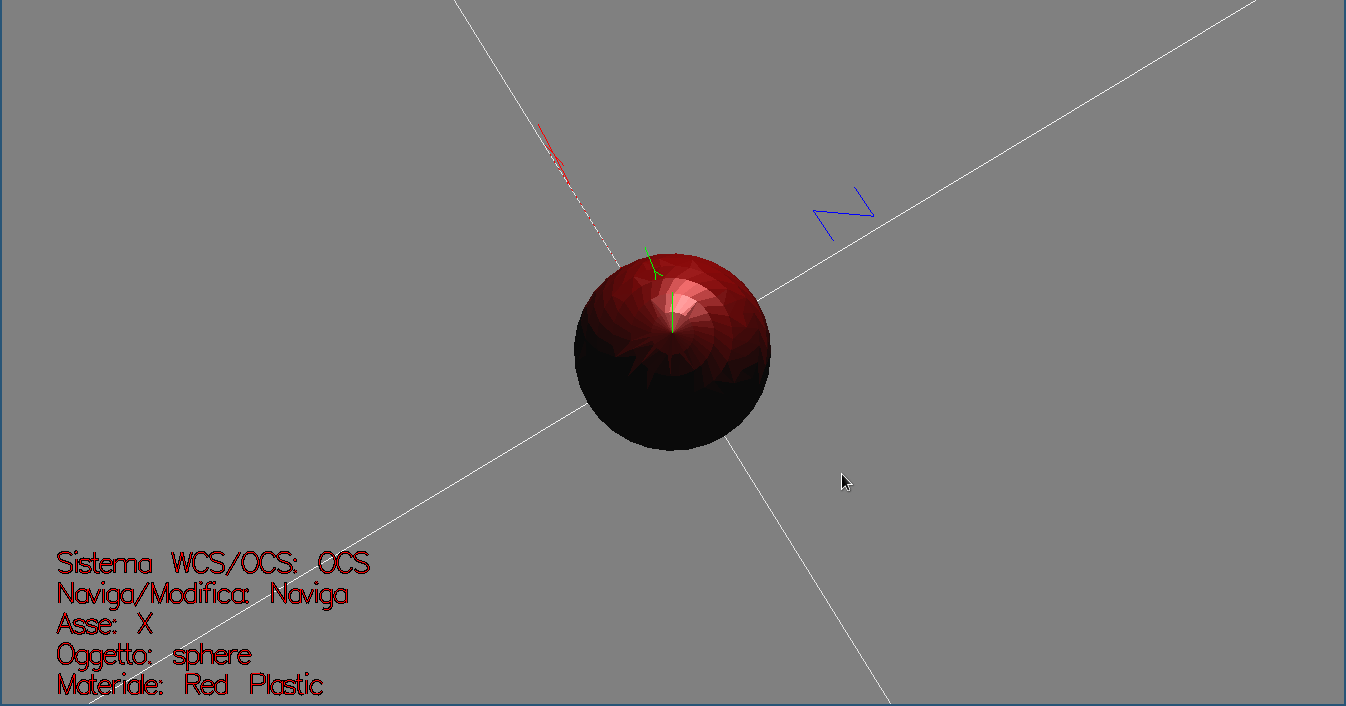
\includegraphics[width=0.6\textwidth]{moveAround.png}} 
    \end{enumerate}
    \item Trasformazione degli oggetti in scena
    \begin{enumerate}
        \item Per ottenere la posizione attuale dell'oggetto, si moltiplica l'identità per la matrice dell'oggetto, per effettuare la traslazione si può utilizzare la funzione \textit{GlTransaltef}, per la rotazione la funzione \textit{glRotatef} e infine per la scalatura \textit{glScalef}. Per questa ultima funzione non ho capito se si dovesse scalare un asse alla volta, oppure no. Personalmente ho preferito implementare la scalatura dell'oggetto in sè, in quanto la consideravo più utile, ma se fosse stato necessario scalare un asse alla volta, è sufficiente modificare i parametri di \textit{glScalef} controllando l'asse di lavoro. La differenza tra WCS e OCS consiste semplicemente nell'ordine delle operazioni svolte, come è possibile verificare nella funzione \textit{modifyModelMatrix}\\
           {\centering
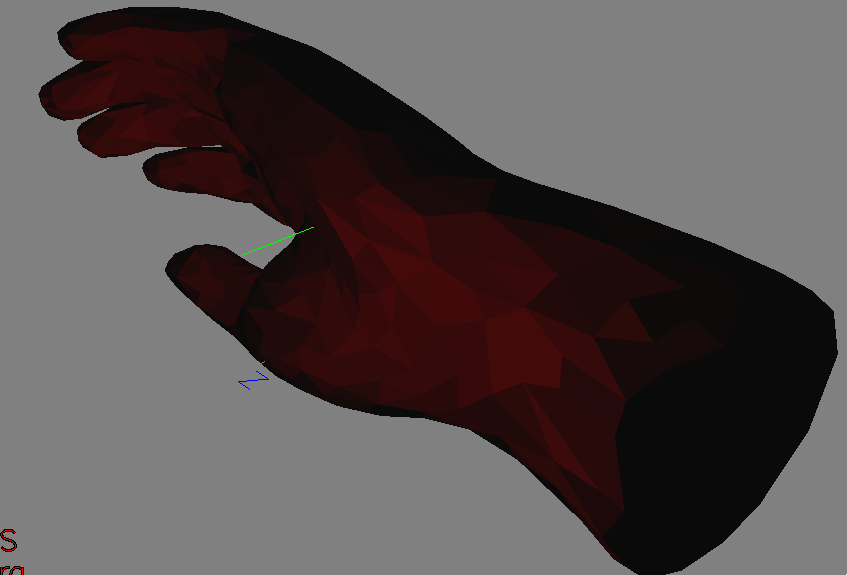
\includegraphics[width=0.6\textwidth]{manoTrasl.png}} 
    \end{enumerate}
    
\end{enumerate}
